\documentclass[a4paper, 12pt]{article}
\usepackage{graphicx}
\usepackage{geometry}
\usepackage{subcaption}
\usepackage{biblatex}
\usepackage{blindtext}
\usepackage{amsmath}
\usepackage[skip=10pt, indent=25pt]{parskip}

\usepackage{multirow}
\usepackage{algorithmicx}
\usepackage[vietnamese]{babel}
\usepackage{multicol}
\setlength{\columnsep}{2cm}
\geometry{
	a4paper,
	left=20mm,
	right=20mm,
	top=20mm,
	bottom=20mm
}
\usepackage{listings}
\lstset{language=Python}

\algdef{SE}[DOWHILE]{Do}{doWhile}{\algorithmicdo}[1]{\algorithmicwhile\ #1}%

\setlength{\parindent}{25pt}
\begin{document}
	\begin{titlepage}
		\centering
		
		\textsc{\Large ĐẠI HỌC QUỐC GIA THÀNH PHỐ HỒ CHÍ MINH}\\
		\vspace{0,2cm}
		\textsc{\Large TRƯỜNG  ĐẠI HỌC KHOA HỌC TỰ NHIÊN}\\
		\vspace{0,2cm}
		\textsc{\large KHOA CÔNG NGHỆ THÔNG TIN}
			
		\begin{centering}
			{
\includegraphics[width=6cm]{logo.png}}
		\end{centering}
		
		% TITLE 
		\begin{center}
			\line(1,0){170mm}
		\end{center}
		\Huge \textbf{BÁO CÁO SEMINAR}\\ 
		\vspace{0.1cm}
		\vspace{0.1cm}
		\Huge \textbf{Cách cài đặt chat bot trên ứng dụng web sử dụng API key của OpenAI} \\
		\begin{center}
			\line(1,0){450}
		\end{center}
		
		\vspace{0,2cm}
		\huge \textbf{Môn học: Mạng Máy Tính}\\
		\Large{\textbf{Giảng viên: Th.S Đỗ Hoàng Cường}}
		\Large
		% AUTHOR
		\vspace{1cm}
		% Please add the following required packages to your document preamble:
		% \usepackage{booktabs}
		\begin{table}[h]
			\centering
			\begin{tabular}{@{}lll@{}}
				& \textbf{Họ và tên}         & \textbf{MSSV} \\
				& Nguyễn Quốc Trung & 21120350 \\
				& Trần Kỳ Thanh     & 21120556 \\
				& Trần Trọng Nghĩa  & 21120507 \\ 
			\end{tabular}
		\end{table}

		
		% DATE
		\vspace{1cm}
		{\scshape \today}
	\end{titlepage}


	\section{Giới thiệu}
		\subsection{ChatGPT}
			Chat bot là một chương trình phần mềm được thiết kế để giao tiếp với con người thông qua hội thoại bằng văn bản, hỗ trợ con người trong nhiều công việc khác nhau như bán hàng, quảng bá sản phẩm, hỗ trợ khách hàng, giới thiệu nội dung...
			\\
			\\
			ChatGPT là một mô hình máy học (machine learning) được phát triển bởi OpenAI, một tổ chức nghiên cứu trí tuệ nhân tạo được thành lập vào năm 2015. ChatGPT gây chú ý bởi khả năng sinh ra văn bản tự nhiên với độ chính xác cao, dưới nhiều hình thức nội dung khác nhau (giải thích kiến thức, soạn e-mail, viết CV...) theo yêu cầu của người dùng cuối. 
			\\
			\\
			GPT là từ viết tắt tiếng Anh của Generative Pre-trained Transformer - một mạng lưới thần kinh AI được huấn luyện với lượng khổng lồ dữ liệu văn bản lấy từ các nguồn đa dạng về nội dung, chủ đề, ngôn ngữ và cấu trúc nhằm giúp mô hình có thể trả về các phản hồi tự nhiên, giống với ngôn ngữ của con người nhất có thể thông qua cơ chế học sâu.
			\\
			\\
			Nền tảng của ChatGPT là mô hình mạng thần kinh (neural network) - một mô hình học sâu được cấu thành từ các neuron nhân tạo (được gọi là nút) tổ chức thành nhiều lớp (mỗi lớp gồm nhiều nút), được liên kết chặt chẽ với nhau. Trong mạng thần kinh, thông tin được truyền đi thông qua mạng lưới kết nối phức tạp giữa các lớp, còn quá trình tính toán cụ thể được thực thi tại từng nút. Nhờ cơ chế này, mô hình dần có được khả năng nhận dạng các mẫu và dấu hiệu lặp đi lặp lại trong dữ liệu đầu vào, từ đó "học" được kiến thức mà người phát triển mong muốn, giúp đưa ra kết quả chính xác và đáp ứng được yêu cầu công việc.
			\\
			\\
			Với 175 tỷ tham số trong mô hình, khối lượng dữ liệu training khổng lồ, ChatGPT đã trở thành một công cụ tiên phong trong công việc xử lý ngôn ngữ tự nhiên và có ảnh hưởng to lớn đến khắp các lĩnh  vực, từ thị trường công nghệ, việc làm, đến giáo dục và đào tạo...
			
		
		\subsection{Những tính năng nổi bật của ChatGPT}
		Một số tính năng nổi bật của ChatGPT bao gồm:
		\begin{itemize}
			\item Giao tiếp cơ bản với người dùng: chào hỏi, hội thoại cơ bản, phản hồi với nhận xét của người dùng.
			\item Trả lời những câu hỏi trực tiếp từ người dùng về hầu hết các chủ đề.
			\item Thông báo với người dùng nếu không có hiểu biết về chủ đề được yêu cầu.
			\item Soạn e-mail theo yêu cầu của người dùng về nội dung, văn phong, hình thức, mục đích.
			\item Đề xuất ý tưởng trong nhiều lĩnh vực như công việc, học tập, giải trí, sáng tạo nội dung.
			\item Viết code theo yêu cầu người dùng và giải thích code.
			\item Có thể dịch văn bản với nhiều ngôn ngữ khác nhau.
			\item Đọc hiểu văn bản: phân tích nội dung, bố cục, văn phong, ngữ nghĩa...
			\item Tạo ra các tác phẩm truyện, thơ, bài viết ngắn, tóm tắt, báo cáo và nội dung khác dựa trên thông tin được cung cấp.
			\item Phân tích dữ liệu và trích xuất thông tin từ các nguồn dữ liệu khác nhau như báo cáo, trang web, tài liệu học tập, tin tức và phương tiện truyền thông xã hội.
			\item Ghi nhớ lịch sử hồi thoại để duy trì đối thoại một cách tự nhiên  nhất có thể và đính chính thông tin sai lệch nếu có.
			\item Từ chối tạo ra các nội dung nhạy cảm, không lành mạnh.
			\item Điều khiển và điều chỉnh các thiết bị thông minh: hỗ trợ người dùng điều khiển các thiết bị thông minh như đèn, máy lạnh, thiết bị giải trí qua các lệnh đơn giản.
		\end{itemize}
		Ngoài ra, ChatGPT vẫn còn tồn tại những vấn đề như:
		\begin{itemize}
			\item Có thể đưa ra thông tin sai lệch, không chính xác.
			\item Có thể hiểu sai yêu cầu hoặc ý định của người dùng và cung cấp phản hồi không chính xác hoặc không phù hợp.
			\item Thiếu khả năng tương tác thực tế: chỉ có thể tương tác với người dùng thông qua văn bản, không có khả năng tương tác trực tiếp với môi trường thực tế.
			\item Thiếu khả năng đánh giá và lựa chọn: ChatGPT hiện tại chưa có khả năng đánh giá và lựa chọn các phương án tối ưu nhất trong các tình huống phức tạp.
			\item Tính bảo mật: nguy cơ rò rỉ thông tin và xâm nhập tài khoản của người dùng.
			\item Khả năng bị lạm dụng: ChatGPT có thể bị lạm dụng để tạo ra các phản hồi giả mạo hoặc các thông tin sai lệch, gây ra những hậu quả tiêu cực cho người dùng và xã hội.
			\item Bị ảnh hưởng bởi thiên kiến của dữ liệu training.
			\item Không có hiểu biết đầy đủ về những sự kiện, hiện tượng xảy ra sau 2021.
		\end{itemize}
	
		
		\subsection{Triển vọng}
		\begin{itemize}
			\item Đẩy mạnh quá trình tương tác giữa người và máy.
			\item Trợ lý ảo và hệ thống tự động.
			\item Tra cứu thông tin, tóm tắt kiến thức, trích dẫn nguồn, kiểm định thông tin.
			\item Tư vấn người dùng về các lĩnh vực cụ thể (y tế, giáo dục, tài chính...).
			\item Hỗ trợ học sinh, sinh viên trong công tác học tập, chuẩn bị bài, nghiên cứu, hoàn thành bài tập.
			\item Hỗ trợ người dùng có các vấn đề sức khỏe, thương tật.
			\item Phát triển các trò chơi thông minh có tính tương tác cao.
			\item Hỗ trợ ngôn ngữ: dịch thuật, giải thích định nghĩa của từ.
		\end{itemize}
	
	\section{Cài đặt chat bot}
		\subsection{Tạo tài khoản OpenAI}
		Hiện tại, Việt Nam chưa có trong danh sách các quốc gia mà OpenAI trực  tiếp hỗ trợ cung cấp dịch vụ. Khi truy cập vào trang web chính thức từ mạng Việt Nam, người dùng sẽ nhận được thông báo "ChatGPT is not available in your country", cho thấy ứng dụng này chưa được hỗ trợ tại quốc gia của chúng ta.
		\\
		\\
		Do đó, giải pháp dành cho người dùng tại Việt Nam là thông qua các kênh thứ ba để đăng ký truy cập như sử dụng VPN để thay đổi sang địa chỉ IP của các nước được hỗ trợ dịch vụ, thuê số điện thoại nước ngoài để đăng ký tài khoản, hay mua các tài khoản có sẵn. 
		\\
		Tuy nhiên, việc sử dụng các kênh thứ ba mang lại một số rủi ro tiềm ẩn nhất định cho người dùng. Ví dụ, việc quá nhiều người cùng sử dụng một tài khoản có thể làm chậm quá trình nhận phản hồi và giảm hiệu quả công việc, thường xuyên gây tắc nghẽn. Ngoài ra, việc thuê số điện thoại nước ngoài hoặc mua tài khoản không uy tín chứa đựng nguy cơ bị lừa đảo. Hơn nữa, người dùng không sở hữu tài khoản thực sự vì số điện thoại đăng ký thuộc về bên thứ ba.
		
	\subsection{Nhận API key}
	\begin{itemize}
		\item[\textbf{Bước 1:}] Truy cập vào trang web platform.openai.com bằng đường link Overview - OpenAI API hoặc beta.openai.com.
		
		\item[\textbf{Bước 2:}] Sử  dụng công cụ VPN (nếu cần thiết) và đăng nhập vào tài khoản OpenAI đã được đăng ký trước đó.
		
		\item[\textbf{Bước 3:}] Sau khi đăng nhập thành công, mở trang chủ platform.openai.com và di chuyển chuột đến mục Personal ở góc trên bên phải màn hình, chọn mục "View API keys".
		
		\begin{centering}
			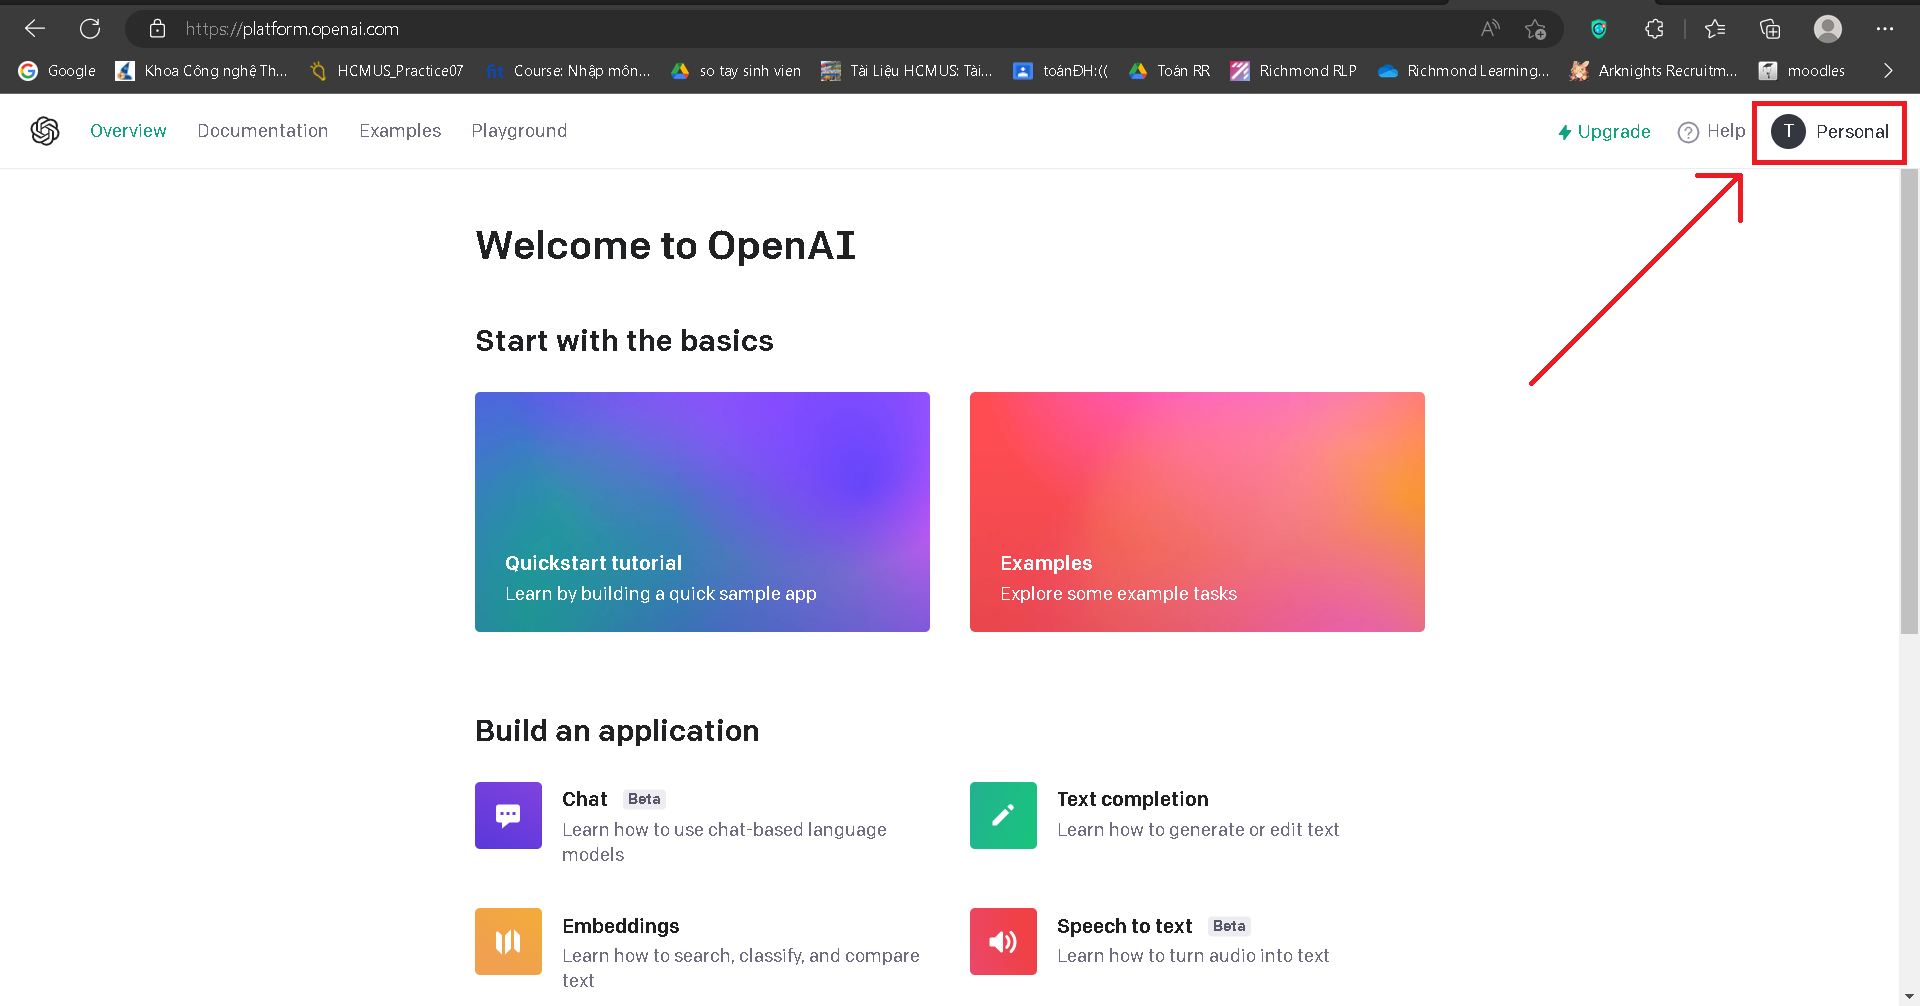
\includegraphics[width = 170mm]{1.png}
			\captionof{figure}{Di chuột vào mục personal để hiện các tùy chỉnh và thông tin cá nhân}	
		\end{centering}
		\begin{centering}
						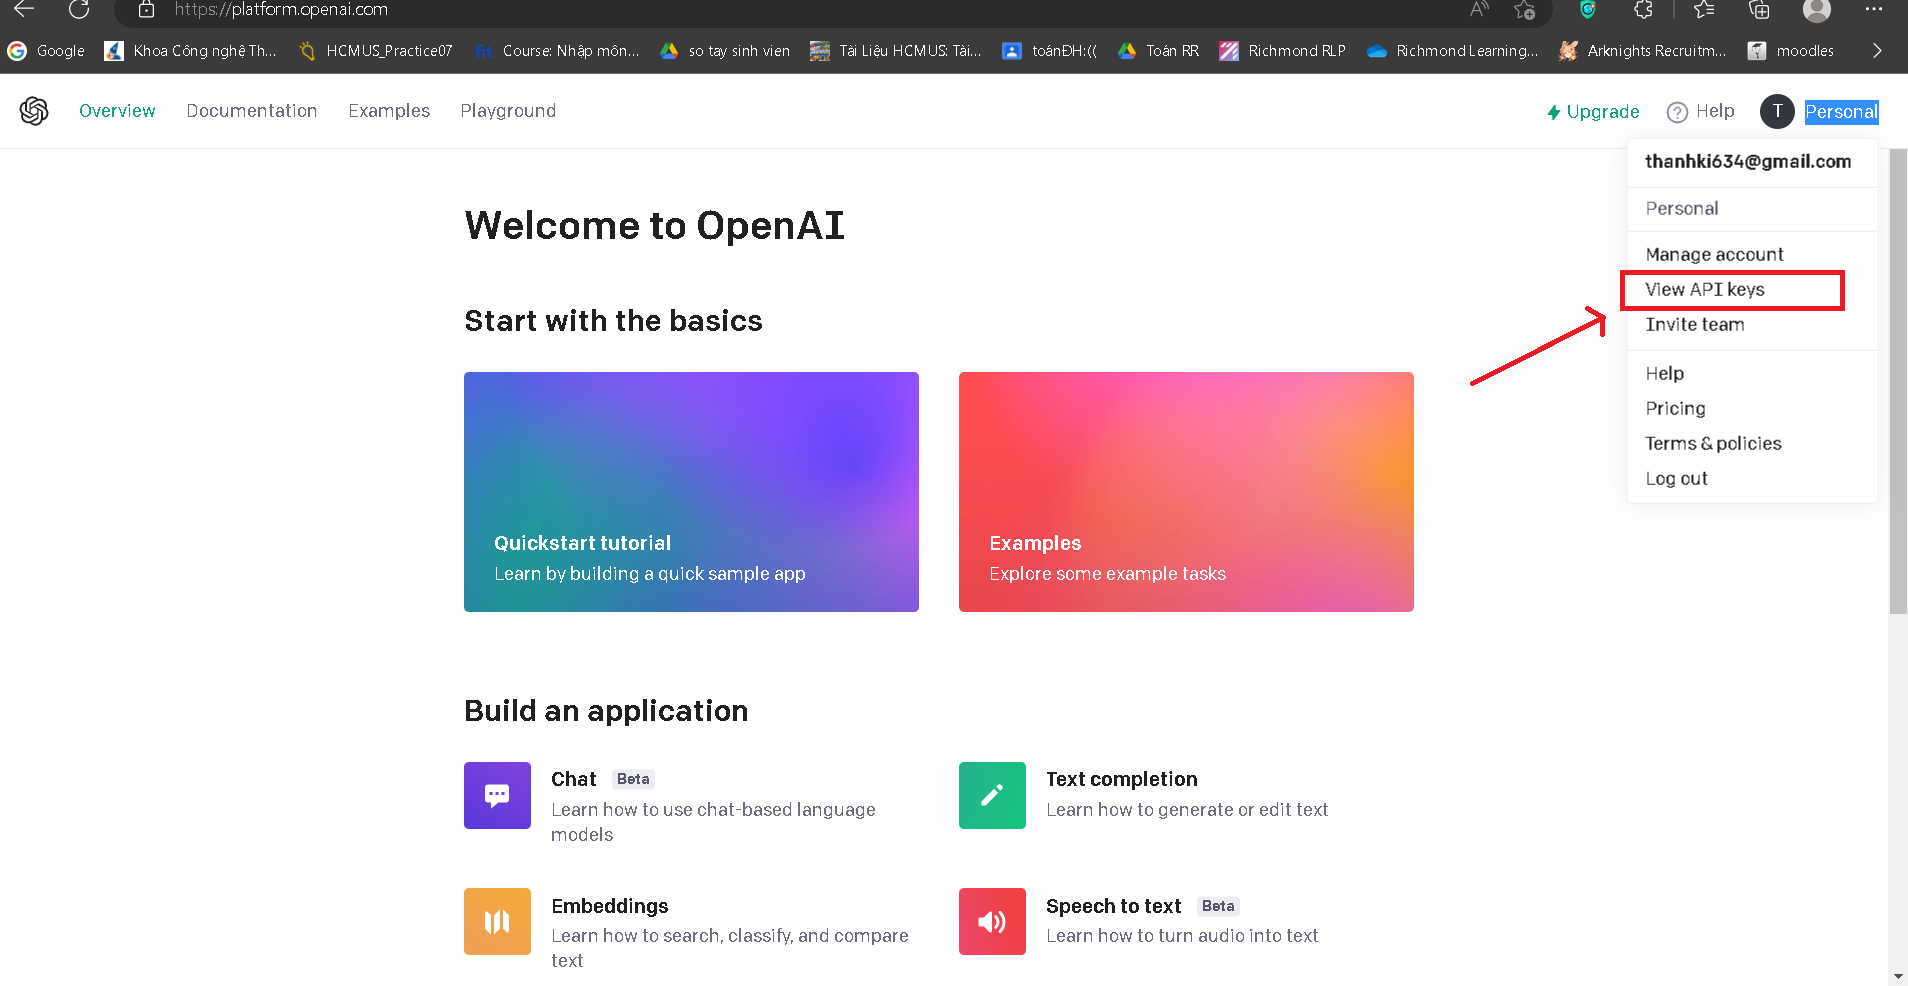
\includegraphics[width = 170mm]{2.png}
			\captionof{figure}{Chọn mục "View API keys" để được đưa đến trang kiểm soát API key}
		\end{centering}
	
		\item[\textbf{Bước 4:}] Bấm vào mục “Create new secret key” để khởi tạo một API key mới. Một  hộp thoại sẽ hiện lên cùng với API key được khởi tạo. Lưu lại API key này ở một nơi an toàn vì sau khi tắt hộp thoại, sẽ không thể xem đầy đủ API key này được nữa.
		
		\begin{centering}
			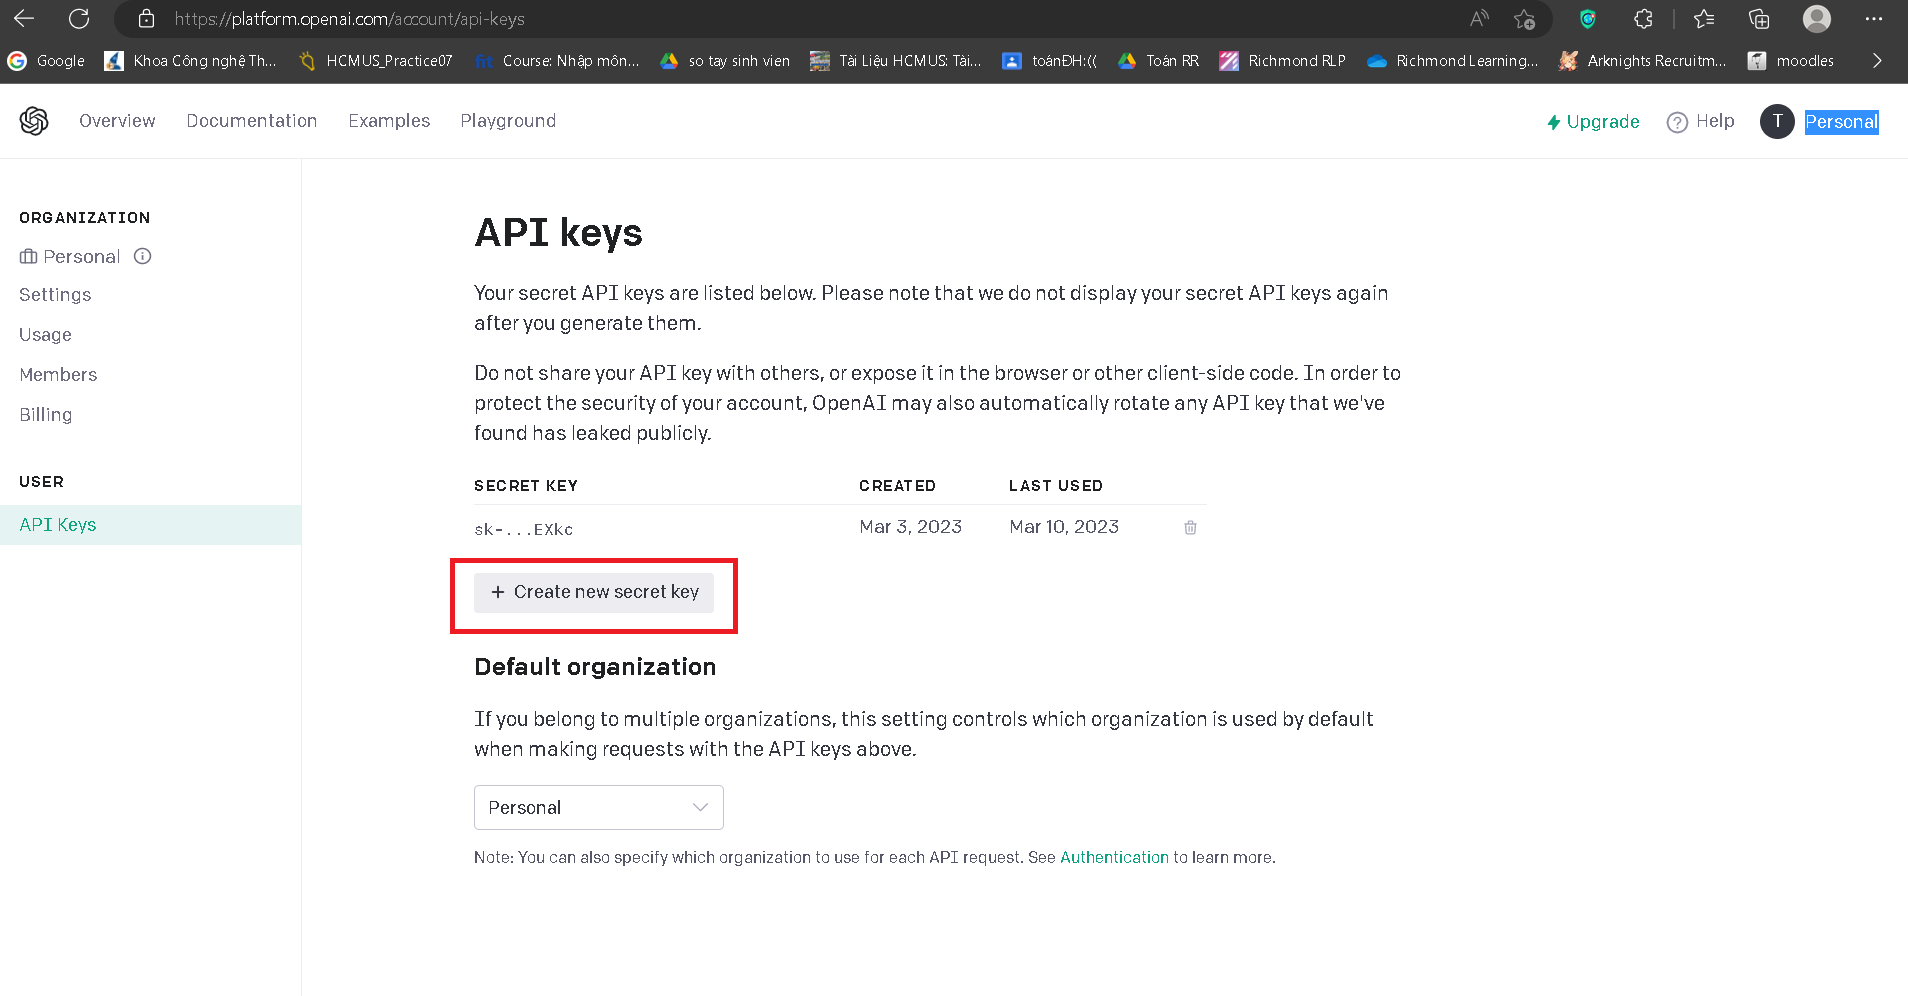
\includegraphics[width = 170mm]{3.png}
			\captionof{figure}{Chọn "Create new secret key" để khởi tạo API key mới}	
		\end{centering}
		\begin{centering}
						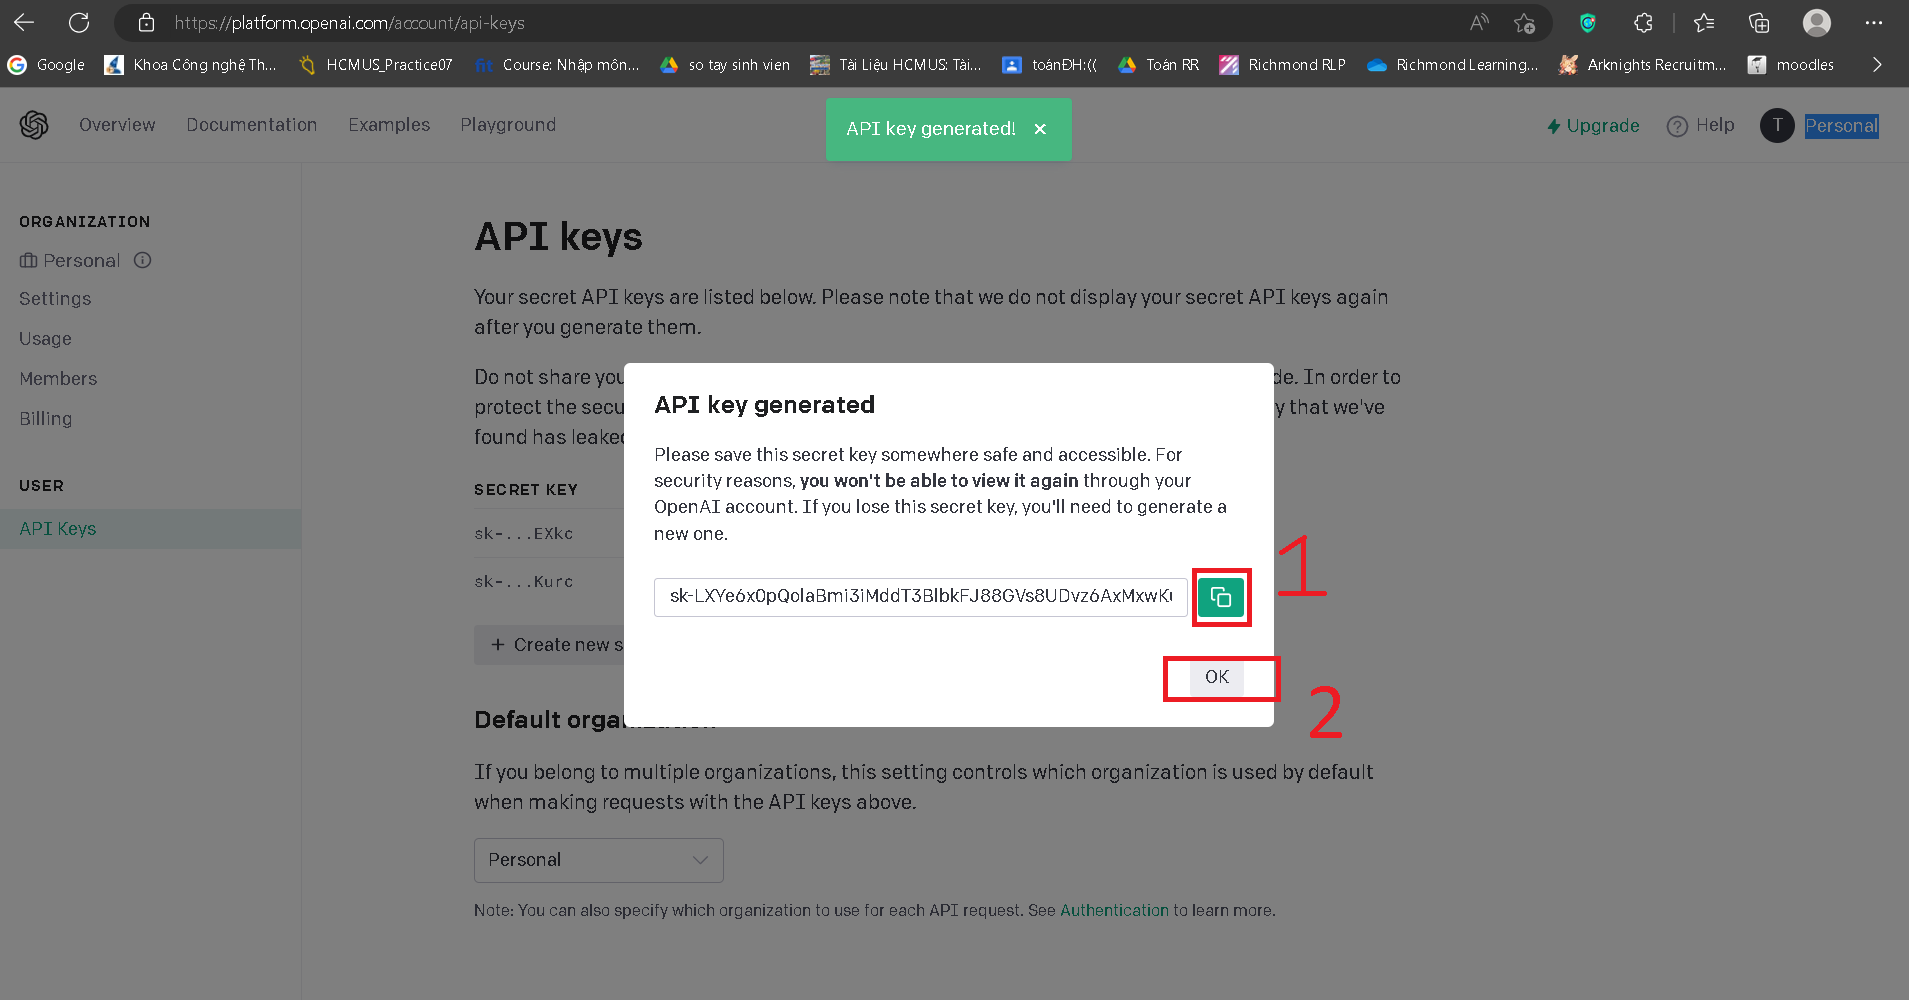
\includegraphics[width = 170mm]{4.png}
			\captionof{figure}{Sao chép key vừa được khởi tạo, lưu nó ở nơi an toàn. Sau đó tắt hộp thoại để hoàn tất quá trình khởi tạo}
		\end{centering}
	\item[\textbf{Lưu ý:}] Một tài khoản miễn phí được cung cấp cho người dùng bởi OpenAI có hạn mức sử dụng là \$18, sau khi sử dụng hết hạn mức và quá thời hạn được quy định trước, người dùng cần nạp thêm tiền vào tài khoản để có thể tiếp tục sử dụng các dịch vụ của OpenAI (Mỗi một lần gọi API key có chi phí \$0.02.)
	\begin{centering}
		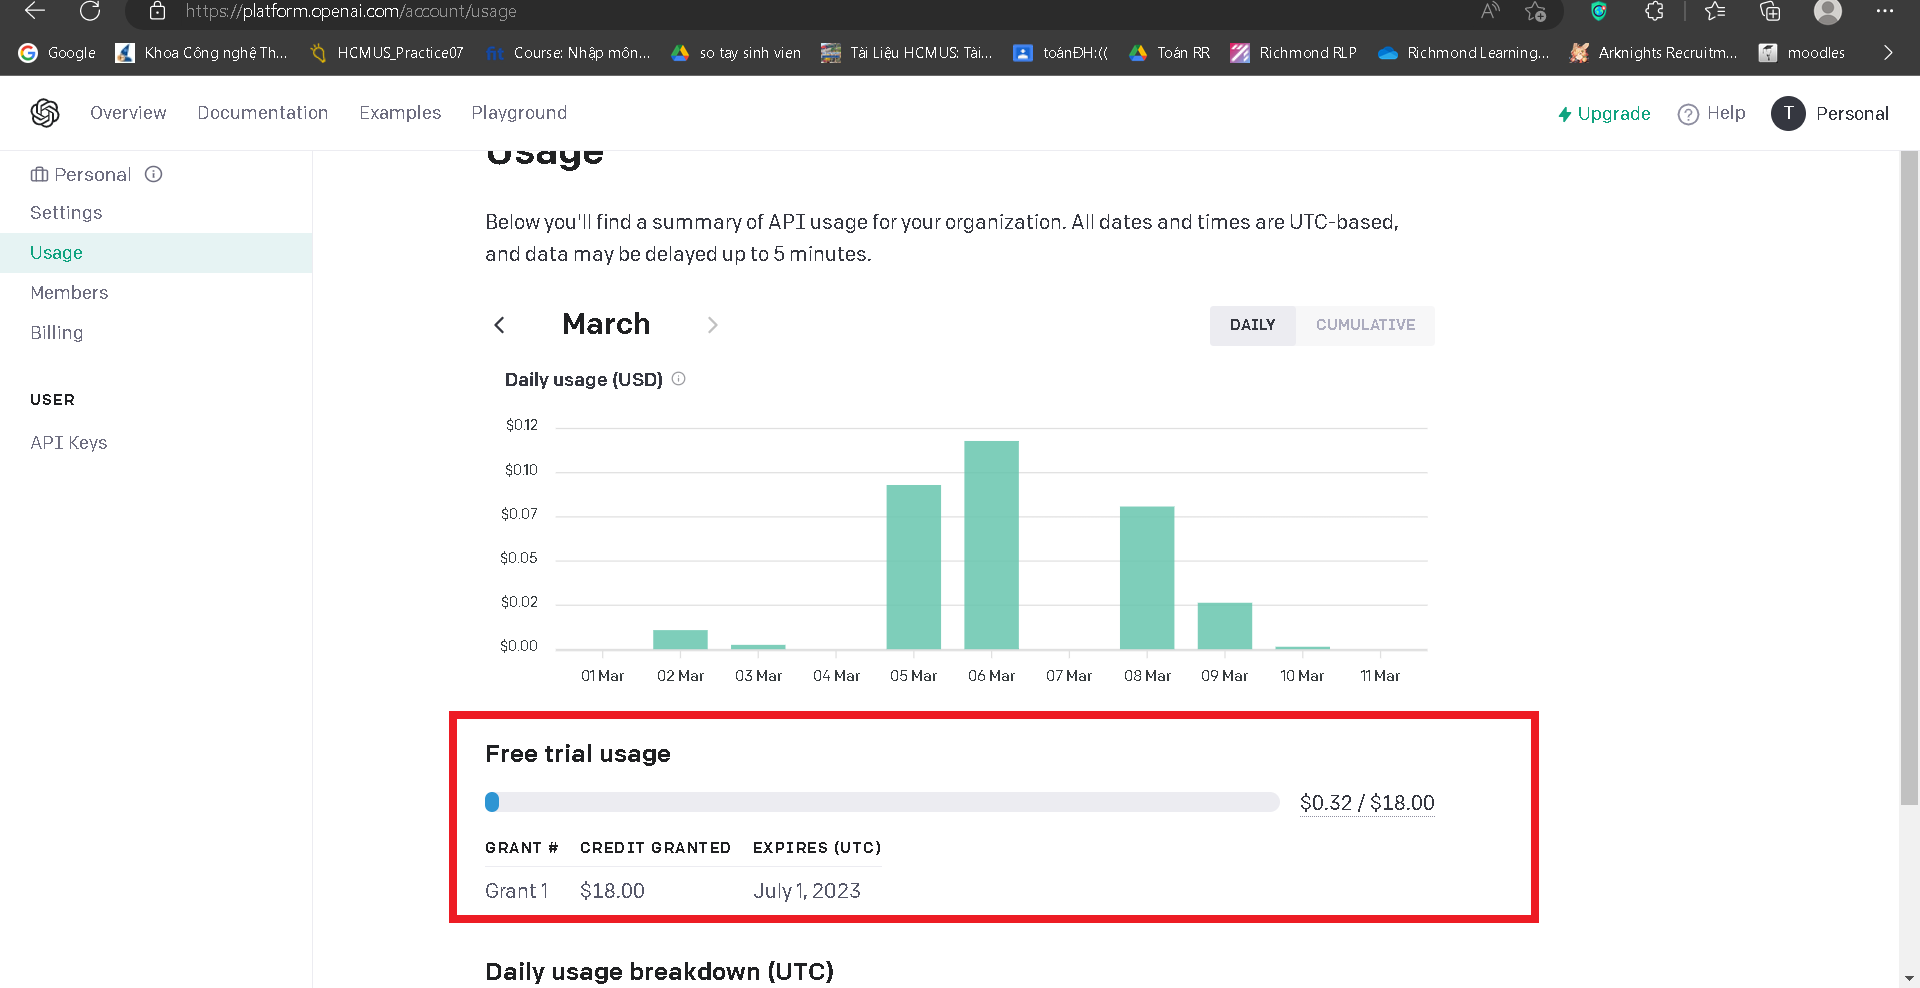
\includegraphics[width = 170mm]{4.5.png}
		\captionof{figure}{Hạn mức sử dụng và thời hạn sử dụng được hiển thị trong\\ platform.openai.com/account/usage}	
	\end{centering}
	\end{itemize}
	
	\section{Cài đặt chat bot}
	Chat bot của chúng tôi được xây dựng trên nền tảng ứng dụng web (sử dụng javascript), và có tham khảo các tài liệu hướng dẫn cũng như một số dự án mã nguồn mở khác có liên quan.
	\subsection{Back-end}
	Back-end của chúng tôi được cài đặt bằng ngôn ngữ javascript, với nhiệm vụ quan trọng nhất là thực hiện gửi yêu cầu HTTP lên điểm cuối của OpenAI và nhận về dữ liệu phản hồi ứng với dữ liệu đã truyền vào. Từ đó, câu trả lời ứng với nội dung nhập của người dùng được tách ra và xuất trên giao diện ứng dụng.
	\\
	\\
	Tổng quan, trình tự hoạt động của back-end khi thực hiện yêu cầu HTTP như sau:
	\begin{itemize}
		\item[1.] Tạo đối tượng lưu giữ yêu cauafw 
	\end{itemize}
	
	
	\subsection{Cấu trúc mã nguồn}
	
	Tổng quan, mã nguồn cài đặt các công việc chính:
	\begin{itemize}
		\item[1.] Khai báo các thư viện sử dụng
		\item[2.] Xác thực API key bằng Key đã được tạo trong đề mục 2.
		
		\item[3.] Thêm dữ liệu đầu vào: Hàm \texttt{add\_request(history, request)} nhận yêu cầu mới của người dùng dưới dạng chuỗi văn bản và chèn yêu cầu này vào cuối biến danh sách \texttt{history} với định dạng mà hàm sinh kết quả hiểu được. 
		\item[4.] Thêm dữ liệu đầu ra: Hàm \texttt{add\_response(history, request)} nhận câu trả lời của AI dưới dạng chuỗi văn bản và  chèn chúng vào cuối biến danh sách \texttt{history} với định dạng mà hàm sinh kết quả  hiểu được. 
		\item[5.] \begin{sloppypar}Hàm sinh kết quả \texttt{generate\_response} nhận vào danh sách lịch sử  hội thoại và nội dung người dùng nhập vào, cập nhật lịch sử hội thoại rồi sau đó gọi hàm \texttt{openai.ChatCompletion.create()} để tạo câu trả lời. Hàm này duyệt qua toàn bộ lịch sử hội thoại được lưu trong \texttt{history} rồi tạo ra câu trả lời cho yêu cầu cuối cùng trong lịch sử hội thoại được sử dụng, đồng thời có thể được tùy chỉnh theo các tham số như model (mô hình), temperature (chỉ số ngẫu nhiên của kết quả)... Kết quả sinh ra được cập nhật trong lịch sử hộp thoại để sử dụng cho lần gọi tiếp theo. \end{sloppypar}
		\item[6.] Hàm \texttt{chat} nhận dữ liệu được nhập vào UI và dữ liệu phát sinh trong quá trình chạy ứng dụng (chính là lịch sử hội thoại), gọi các hàm đã giải thích ở trên, rồi lưu vào biến lưu trữ để ứng dụng xử lý tiếp.
		\item[7.] Hàm tạo UI với khung nhập liệu, khung hiển thị lịch sử hội thoại. Khi kích hoạt, chúng sẽ gọi hàm \texttt{chat} với tham số là các biến lưu dữ liệu .
	\end{itemize}
	\subsection{Nhận xét}
	\textbf{Chức năng}\\
	\begin{itemize}
		\item Có thể vận hành như 1 chat bot cơ bản, trả lời được đa số các câu hỏi đưa ra một cách rõ ràng, mạch lạc với độ tin cậy cao.
		\item Kết quả được trình bày thành trên đoạn, nhiều dòng.
		\item Định dạng riêng cho code.
		\item Có thể nhớ lịch sử hội thoại để tiếp tục nhận phản hồi, tiếp tục chủ đề được đề cập đến mà không bị ngắt quãng.
	\end{itemize}
	\vspace{1,5cm}
	\textbf{Khuyết điểm}\\
	\begin{itemize}
		\item Thỉnh thoáng sẽ xuất hiện lỗi ngữ pháp, câu cú.
		\item Chỉ có duy nhất một khung chat.
		\item Không thể hủy quá trình sinh câu trả lời giữa chừng.
	\end{itemize}
		
	\section{Tham khảo}
	\begin{itemize}
		\item[ {[1]} ] \textit{Introducing ChatGPT}. OpenAI. Truy cập ngày 12 tháng 3 năm 2023.\\ https://openai.com/blog/chatgpt 
		
		\item[ {[2]}] \textit{Definition: GPT-3}. TechTarget. Truy cập ngày 12 tháng 3 năm 2023.\\
		https://www.techtarget.com/searchenterpriseai/definition/GPT-3
		
		\item[{[3]}] \textit{What is deep learning?}. IBM. Truy cập ngày 12 tháng 3 năm 2023.\\
		https://www.ibm.com/topics/deep-learning
		
		\item[{[4]}] \textit{What are neural networks?}. IBM. Truy cập ngày 12 tháng 3 năm 2023.\\
		https://www.ibm.com/topics/neural-networks
		
		\item[{[5]}] \textit{API reference}. OpenAI. Truy cập ngày 12 tháng 3 năm 2023.\\
		https://platform.openai.com/docs/api-reference/
		
		\item[{[6]}] Hamilton, A.C. (2022) \textit{How to Create an  Advanced Chatbot: A Comprehensive Guide to Using Open AI's Chat GPT}. Digital Age Media.
		
		
			
	\end{itemize}
\end{document}